\documentclass[12pt]{article}

\usepackage{sbc-template}

\usepackage{graphicx,url}
%\usepackage{subcaption}
\usepackage{subfigure}

\usepackage[brazil]{babel}
\usepackage[utf8]{inputenc}  

\hfuzz=0.64pt
\sloppy

\title{Implementa\c{c}\~ao do k-nearest neighbors -- KNN\\ em VHDL}

\author{Alexandre G. da Costa\inst{1}, Diego P. Jaccottet\inst{1}, Leandro W.
  Dias\inst{1} }


\address{CDTec -- Universidade Federal de Pelotas
  (UFPEL)\\
  CEP 96.010-610 -- Pelotas -- RS -- Brazil
  \email{alexandre.costa@inf.ufpel.edu.br, \{diego.porto.j,lwdias\}@gmail.com}
}

\begin{document} 

\maketitle

%\begin{abstract}
%  This paper describes ...
%\end{abstract}
     
\begin{resumo}

Neste trabalho foi implementado o algoritmo KNN na placa Altera Cyclone (2C35)
FPGA de 35.000 LEs, afim de reconhecer indivíduos. Sendo que a entrada é o
esqueleto do indivíduo, esse esqueleto é inferido a partir de filmagem 
tridimensional realizada pelo Kinect Versão 2 no seu SDK. Foi obtido sucesso em
capturar frames, enviar pela porta serial até a placa e mostrar em qual classe,
de uma serie de classes pré definidas, a posição atual da pessoa se encontra.

\end{resumo}

\section{Introdu\c{c}\~ao}

FPGAS são muito usadas para protótipos, onde não se justifica um projeto ASIC
personalizado. Entre as vantagens das FPGAS estão o alto paralelismo e
adaptabilidade, com paralelismo para dados, tarefas, pipeline ou uma mistura
desses. FPGAS também são muito eficientes na questão da quantidade de bits
necessários para uma tarefa. Em FPGAS a lógica de instruções e de-codificação
de endereços se torna desnecessária, isso possibilita alcançar throughput muito
maior que em processadores tradicionais, assim como uma redução da quantidade
de energia usada. FPGAS vem se tornando cada vez mais poderosas, o que torna
seu uso cada vez mais interessante \cite{najjar2003high}.

O uso de gestos é um dos meios de Interação Humano-Computador (Human-Computer-
Interaction - HCI) mais naturais e intuitivos. Além disso existem aplicações em
realidade virtual, linguagem de sinais, e jogos de computador. Criar sistemas
para o reconhecimento de gestos ainda é um problema desafiador. Métodos usando
imagens de profundidade vem se tornando cada vez mais populares, pois é mais
robusto ao fundos de imagem confusos \cite{ren2011robust}. O uso do Kinect pode
simplificar muitas das etapas no processamento de vídeos, já que ele captura e
pré-processa as imagens \cite{Andersson:2014}.

\section{Trabalhos relacionados}

Choi alcançou 89\% de acurácia em 2014 para o reconhecimento de gestos humanos
usando redes neurais \cite{choi2014design}. Zhang alcançou acurácia de 99.14\%
usando SVMs \cite{zhang2014novel}. Saha alcançou 90.83\% usando ensemble trees
\cite{saha2014study}. Os trabalhos usaram uma média de 6 poses. O diferencial
do nosso trabalho está no uso da FPGA.

\section{Kinect Vers\~ao 2} \label{sec:kinectversion2}

O Kinect é um sensor equipado de uma câmera RGB, um sensor de profundidade
composto de um emissor de luz infravermelho e uma câmera sensível à
profundidade.

O principio básico por trás do sensor de profundidade do Kinect é a emissão de
um padrão de infravermelho e a captura simultânea da imagem desse infravermelho
com uma câmera tradicional equipada com um filtro, que permite capturar o 
infravermelho e bloquear outras formas de onda. O processador de imagens do 
Kinect usa as posições relativas dos pontos 
no padrão do infravermelho para calcular o deslocamento da profundidade em cada
posição de pixel na imagem.

Cada pixel do mapa de profundidade representa a distância cartesiana, em 
milímetros, do plano da câmera até o objeto mais próximo, naquela coordenada
(x, y) em particular. Se o valor do pixel é 0, isso indica que o sensor não 
encontrou nenhum objeto no seu espaço de alcance naquela localização (x, y).
Essa projeção é mencionado como espaço de profundidade. Os valores correntes de
profundidade são as distâncias do plano da câmera, ao invés das do sensor 
propriamente dito.

\section{Algoritmo KNN}

O algoritmo de aprendizado supervisionado KNN é utilizado para classificar um
objeto não rotulado, baseado no rótulo de seus vizinhos mais próximos em um
espaço de exemplos \cite{Andersson:2014}. Essa proximidade é, frequentemente,
baseada em uma métrica de distância entre dois pontos, por  exemplo, a
distância Euclidiana. De maneira simplificada, a regra de classificação do KNN
é associar a uma amostra de teste, o rótulo da maioria das categorias de seus
``k'' vizinhos mais próximos.

Um conjunto de treino X consiste em n pares de vetores e rótulos, dispersos em
um espaço de classes. Dado um novo par (x; $\theta$), onde apenas a medida x é
observável, o valor de $\theta$	é estimado pela utilização dos dados contidos
no conjunto X com os vetores e rótulos já conhecidos (supervisionado). Um vetor
x' é um vizinho mais próximo de x, se segundo a Equação:

$d(x_{n}', x) = min(x_i, x) i = 1, 2, ...,n$

A distância mínima entre um vetor vizinho e o vetor testado são iguais ao 
conjunto de distâncias mínimas entre os outros vetores e o vetor testado. 
Normalmente, o ``voto'' do vizinho possui um peso, de acordo com a distância do
vetor testado e seus ``k'' vizinhos mais próximos. Assim, $\theta$ é estimado 
com o rótulo desses ``k'' vizinhos mais próximos,como mostra a 
Figura~\ref{fig:fig1}.

\begin{figure}[!hb]
	\centering
	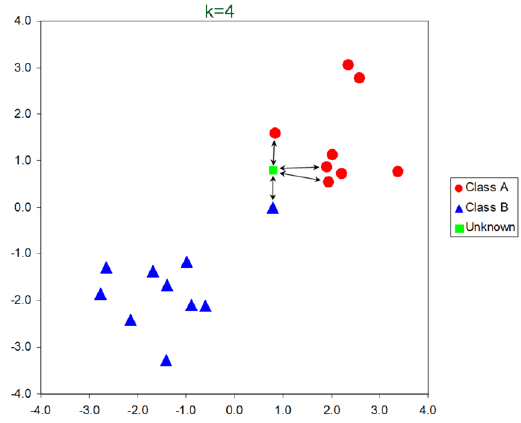
\includegraphics[width=.3\textwidth]{img/knn.png}
	\caption{representação visual de 19 vetores rotulados com classe A e B e uma
	classe desconhecida. O vetor com classe desconhecida é portanto, rotulado
	com seus 4 (k=4) vizinhos mais próximos de acordo com a distância euclidiana
	entre eles.}
	\label{fig:fig1}
\end{figure}

\section{Comunicação serial}

RS-232 é uma comunicação full-duplex(ida e volta ao mesmo tempo). Os sinais são
representados com voltagens em relação ao ground(chamado common). Ele possui 
muitas linhas de handshaking. O sinal muitas vezes está entre -12V e +12V,
sendo -3V e +3V usados para absorver ruídos.

Os sinais na Cyclone para comunicação serial são \verb|UART_TXD| para envio e
\verb|UART_RXD| para receber. O protocolo de comunicação é ilustrado na 
figura~\ref{simulacao}. Cada pacote possui 10 bits, 8 bits de dado e dois para
start e stop. Além disso é necessário um prescaler no código que implementa esse
protocolo, ele deve contar de 0 até 5208, já que 50MHz/9600 Bit/sec = 5208. 9600
é o baud rate da serial. Assim sabemos o tempo que se deve aguardar na contagem,
usando o clock, para igualar o baud rate. Esse método é muito usado em FPGAs
para fazer o timing com unidades externas, como memória RAM, etc.

\begin{figure}[!h]
\centering
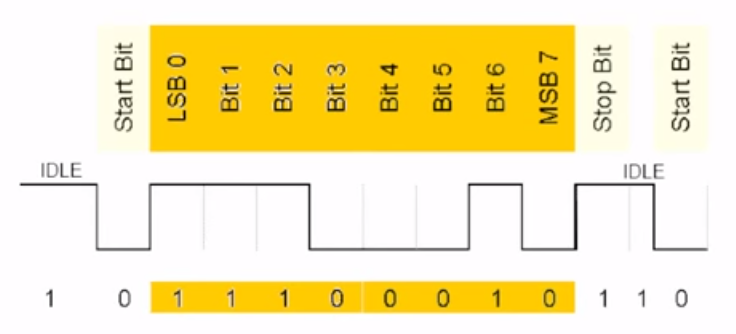
\includegraphics[width=3.3in]{img/uart.png}
% where an .eps filename suffix will be assumed under latex, 
% and a .pdf suffix will be assumed for pdflatex; or what has been declared
% via \DeclareGraphicsExtensions.
\caption{Esquema de transmissão serial.}
\label{simulacao}
\end{figure}

\section{Processo de implementação do algoritmo KNN em VHDL}

O algoritmo usado na implementação VHDL foi o KNN pela distancia euclidiana. 
Esta é a distância entre dois pontos, que pode ser provada pela aplicação
repetida do teorema de Pitágoras \cite{wiki:ieee754en}. A distancia euclidiana
entre o ponto P($p_1, p_2, p_3, ..., p_n$) e Q($q_1, q_2, q_3, ..., q_n$) é
dada por:

$d(p, q) = \sqrt{\sum\limits_{i=1}^n (q_i - p_i)^2}$

Para facilitar a implementação em VHDL, foi considerado K igual a um. 

Os pontos recebidos pela parte de aquisição de dados vem no padrão IEEE 754. O
padrão 754 define regras de operação e representação sobre números binários em
ponto flutuante. Para que o número esteja normalizado deve estar no formato da
Figura~\ref{fig:ieee754ps}.

\begin{figure}[h]
\centering
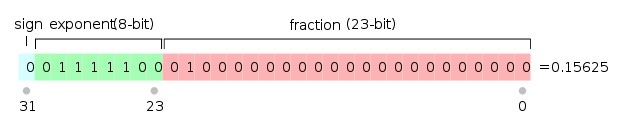
\includegraphics[width=.5\textwidth]{img/IEEE_754_Single_Floating_Point_Format}
\caption{Distribuição dos bits. Precisão simples \cite{wiki:ieee754en}}
\label{fig:ieee754ps}
\end{figure}

A precisão de representação numérica utilizada neste trabalho foi a precisão 
simples. Onde possui 32 bits que em representação seriam 7 digitos decimais.
Destes 32 bits 1 bit é para o sinal, 8 bits para o expoente e 23 bits para 
representar a mantissa.

\subsection{Descrição dos sinais das entradas e saídas}

A figura~\ref{fig:visaogeral} é uma visão geral da comunicação entre o Kinect e
o FPGA.

\begin{figure}[h]
\centering
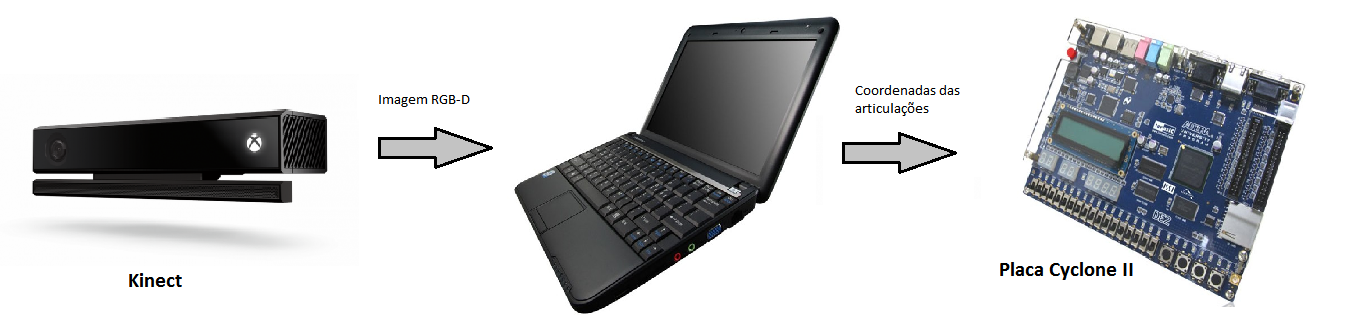
\includegraphics[width=.5\textwidth]{img/visao_geral}
\caption{Visão geral}
\label{fig:visaogeral}
\end{figure}


\begin{itemize}

\item \verb|clock|: é um pino de entrada para prover o sincronismo entre as
operações aritimeticas.

\item \verb|reset|: é um pino de entrada que reinicia o processo de calculo do
KNN. quando esta em 0 os registradores são reiniciados e a maquina de estados
vai para o estado inicial.

\item \verb|uart_rxd|:

\item \verb|key|:

\item \verb|uart_txd|:

\item \verb|end_knn_out|: é um pino de saída que sinaliza quando 
terminou o calculo do KNN.

\item \verb|alb_out|:

\end{itemize}

\subsection{Descrição do bloco operativo}

O bloco operativo é dividito basicamente em 3 loops, onde o primeiro loop vai
acumular os valores e o segundo loop serve apenas para estabilizar o calculo da
raiz quadrada. Quando este processo fica pronto o valor é comparado e
armazenado em um registrador. O terceiro loop serve para carregar o priximo
exemplo armazenado na memória e termina quando não existem mais exemplos para
serem comparados.

Para implementar este processo foram usados uma memória, um subtrator, um 
multiplicador, dois somadores, um acumulador, um bloco que calcula a raiz 
quadrada e um registrador.
Na implementação das operações e da memória foram utilizadas as 
\textit{megafunctions} para ponto flutuante do Quartus II.

\begin{figure}[h]
\centering
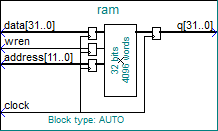
\includegraphics[width=.3\textwidth]{../apresentacao/ram}
\caption{\textit{Megafunction} ``RAM: 1-PORT''}
\label{fig:ram}
\end{figure}

A figura~\ref{fig:ram} descreve uma memória criada pelo 
\textit{MegaWizard Plug-In Manager} do Quartus II. 

O modelo utilizado no trabalho tem as seguintes entradas:
\begin{itemize}
\item \textit{data}~(32 bits): armazena o dado;
\item \textit{wren}~(1 bit): controla a escrita da memória;
\item \textit{address}~(11 bits): endereço de onde vai ser armazenado o dado;
\item \textit{clock}~(1 bit): relógio para sincronizar.
\end{itemize}

Este modelo de memória tem apenas uma saída de dados (q), que tem 32 bits e seu
valor depende da entrada \textit{address}. A memória é inicializada com
exemplos pelo componente \textit{altsyncram} atribuindo a entrada
\verb|init_file| um arquivo ``.mif''.

\begin{figure}[h]
\centering

\subfigure[ALTFP\_ADD\_SUB]{
	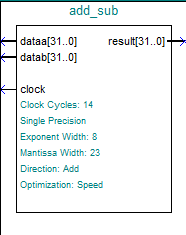
\includegraphics[width=.3\textwidth]{../apresentacao/add_sub}
	\label{fig:add_sub}
}
\quad
\subfigure[ALTFP\_MULT]{
	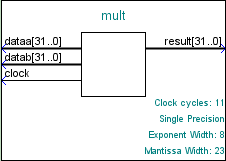
\includegraphics[width=.3\textwidth]{../apresentacao/mult}
	\label{fig:mult}
}
% Você pode adicionar mais subfigures aqui!
\label{fig:addsubmult}
\caption{\textit{Megafunctions} de soma/subtração e multiplicação}
\end{figure}

A figura~\ref{fig:add_sub} descreve a \textit{megafunction} de soma e subtração de
ponto flutuante do Quartus II. Ela foi configurada com formato de precisão
simples de ponto flutuante. Foi utilizado uma latência de 14 ciclos de relógio.

Para fazer a exponenciação foi utilizado um multiplicador de ponto flutuante a
partir da \textit{megafunction} \verb|ALTFP_MULT|. 
A figura~\ref{fig:mult} descreve a \textit{megafunction} de multiplicação de
ponto flutuante do Quartus II. Ela foi configurada com formato de precisão
simples de ponto flutuante. Foi utilizado uma latência de 11 ciclos de relógio.


As \textit{megafunctions} da figura~\ref{fig:addsubmult} foram utilizadas na 
implementação e tem as seguintes entradas:
\begin{itemize}
\item \textit{dataa} e \textit{datab}~(32 bits): dados a serem operados;
\item \textit{clock}~(1 bit): relógio para sincronizar.
\end{itemize}

Esta \textit{megafunction} tem apenas uma saída de resultado (\textit{result})
que tem 32 bits.

\begin{figure}[h]
\centering
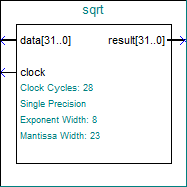
\includegraphics[width=.3\textwidth]{../apresentacao/sqrt}
\caption{\textit{Megafunction} ALTFP\_SQRT}
\label{fig:sqrt}
\end{figure}

A figura~\ref{fig:sqrt} descreve a \textit{megafunction} de raiz quadrada de
ponto flutuante do Quartus II. Ela foi configurada com formato de precisão
simples de ponto flutuante. Foi utilizado uma latência de 28 ciclos de relógio.

A \textit{megafunction} \verb|ALTFP_SQRT| utilizada no trabalho tem as
seguintes entradas:
\begin{itemize}
\item \textit{data}~(32 bits): dado a serem operados;
\item \textit{clock}~(1 bit): relógio para sincronizar.
\end{itemize}

Esta \textit{megafunction} tem apenas uma saída de resultado (\textit{result})
que tem 32 bits.


A figura~\ref{fig:compare} descreve a \textit{megafunction} de comparação de
ponto flutuante do Quartus II. Ela foi configurada com formato de precisão
simples de ponto flutuante. Foi utilizado uma latência de 3 ciclos de relógio.

\begin{figure}[h]
\centering
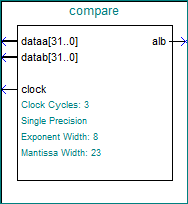
\includegraphics[width=.3\textwidth]{../apresentacao/compare}
\caption{\textit{Megafunction} ALTFP\_COMPARE}
\label{fig:compare}
\end{figure}

A \textit{megafunction} \verb|ALTFP_COMPARE| utilizada no trabalho tem as
seguintes entradas:
\begin{itemize}
\item \textit{dataa} e \textit{datab}~(32 bits): dados a serem operados;
\item \textit{clock}~(1 bit): relógio para sincronizar.
\end{itemize}

Esta \textit{megafunction} tem apenas uma saída que retorna um se a entrada
\textit{dataa} é menor do que a \textit{datab} caso contrario retorna zero.

\begin{figure}[h]
\centering
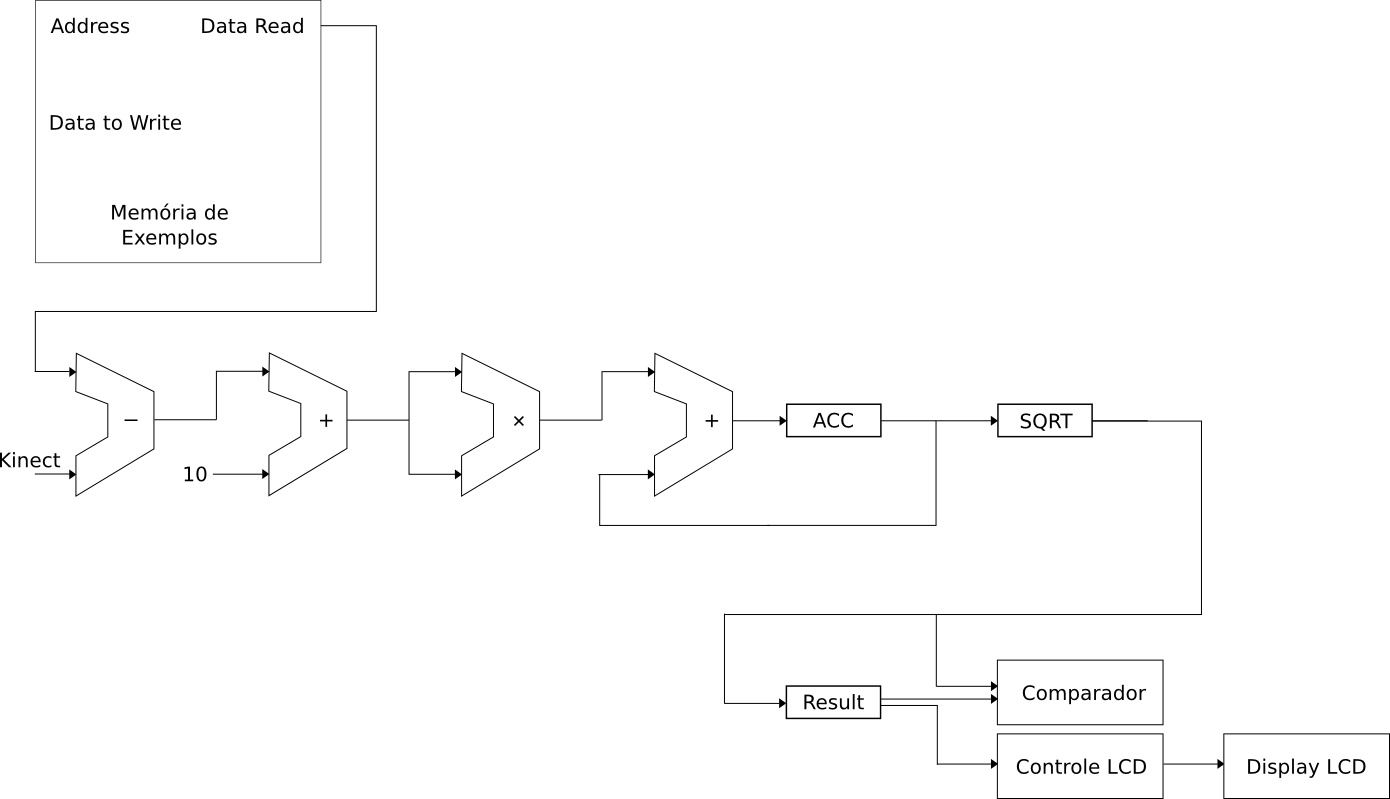
\includegraphics[width=.7\textwidth]{../apresentacao/knn_sem_controle}
\caption{Bloco operativo}
\label{fig:blocoperativo}
\end{figure}

A figura~\ref{fig:blocoperativo} apresenta o bloco operativo. O caminho de
dados inicia quando o bloco de aquisição de dados envia um sinal de que o 
\textit{array} com o frame do Kinect já esta preenchido.


\subsection{Descrição do bloco de controle}

O bloco de controle é composto por 12 estados chamados de \verb|initial|,
\verb|load_memory|, \verb|iterate_lm|, \verb|acc_reset|,
\verb|arith|, \verb|iterate_arith|, \verb|acc_load|, \verb|sqrt|,
\verb|iterate_sqrt|, \verb|result_load|, \verb|iterate| e 
\verb|final|.

Cada estado tem a seguinte funcionalidade:

\begin{itemize}
\item \verb|initial|: responsável por resetar as variáveis e também por esperar os dados vindos do Kinect;
\item \verb|load_memory| e \verb|iterate_lm|: Aguardam a inserção dos exemplos na memória;
\item \verb|acc_reset|: Reseta o registrador do acumulador;
\item \verb|arith| e \verb|iterate_arith|: Estado da realização das operações matemáticas das distâncias euclidianas;
\item \verb|acc_load|: Armazena a soma temporária da distância euclideana no registrador;
\item \verb|sqrt| e \verb|iterate_sqrt|: Realiza o cálculo da raiz quadrada da distância euclideana;
\item \verb|result_load|: Utiliza o componente comparador e carrega o resultado da distância euclideâna no registrador de resultado;
\item \verb|iterate|: Gerencia se o próximo estado será retornar para o "arith" e continuar calculando ou se já terminou os cálculos;
e deve-se ir para o estado "final";
\item \verb|final|: Mostra o resultado na placa e informa a interface com o KNN que a próxima entrada já pode ser enviada.
\end{itemize}

\begin{figure}[!ht]
\centering
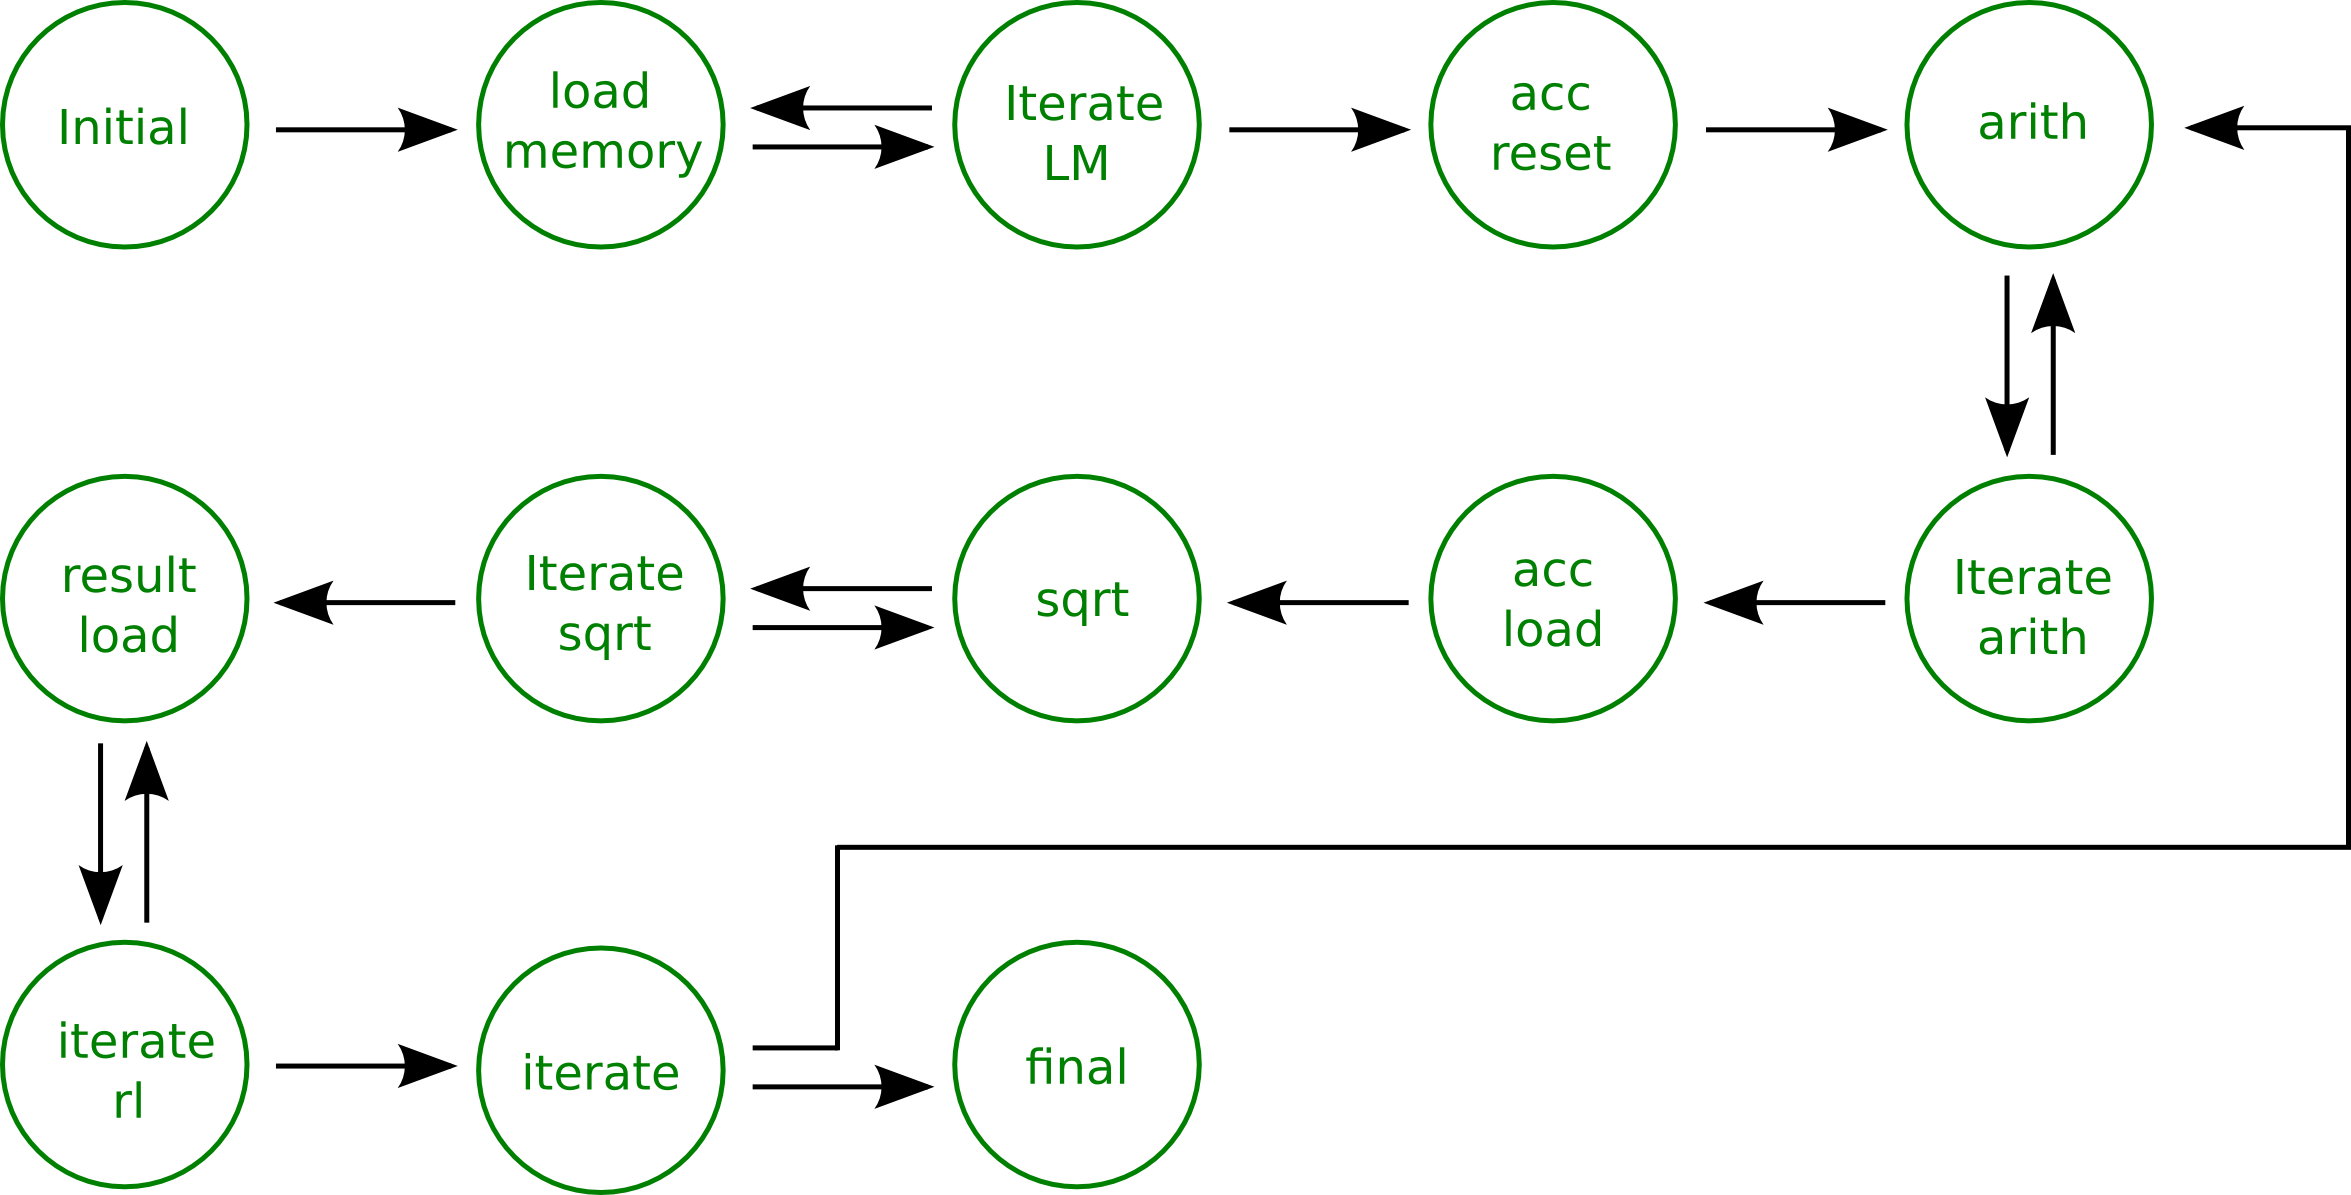
\includegraphics[scale=0.2]{img/control_unit.png}
\end{figure}

\newpage

Abaixo está apresentado o bloco operativo juntamente com o bloco de controle:

\begin{figure}[!ht]
\centering
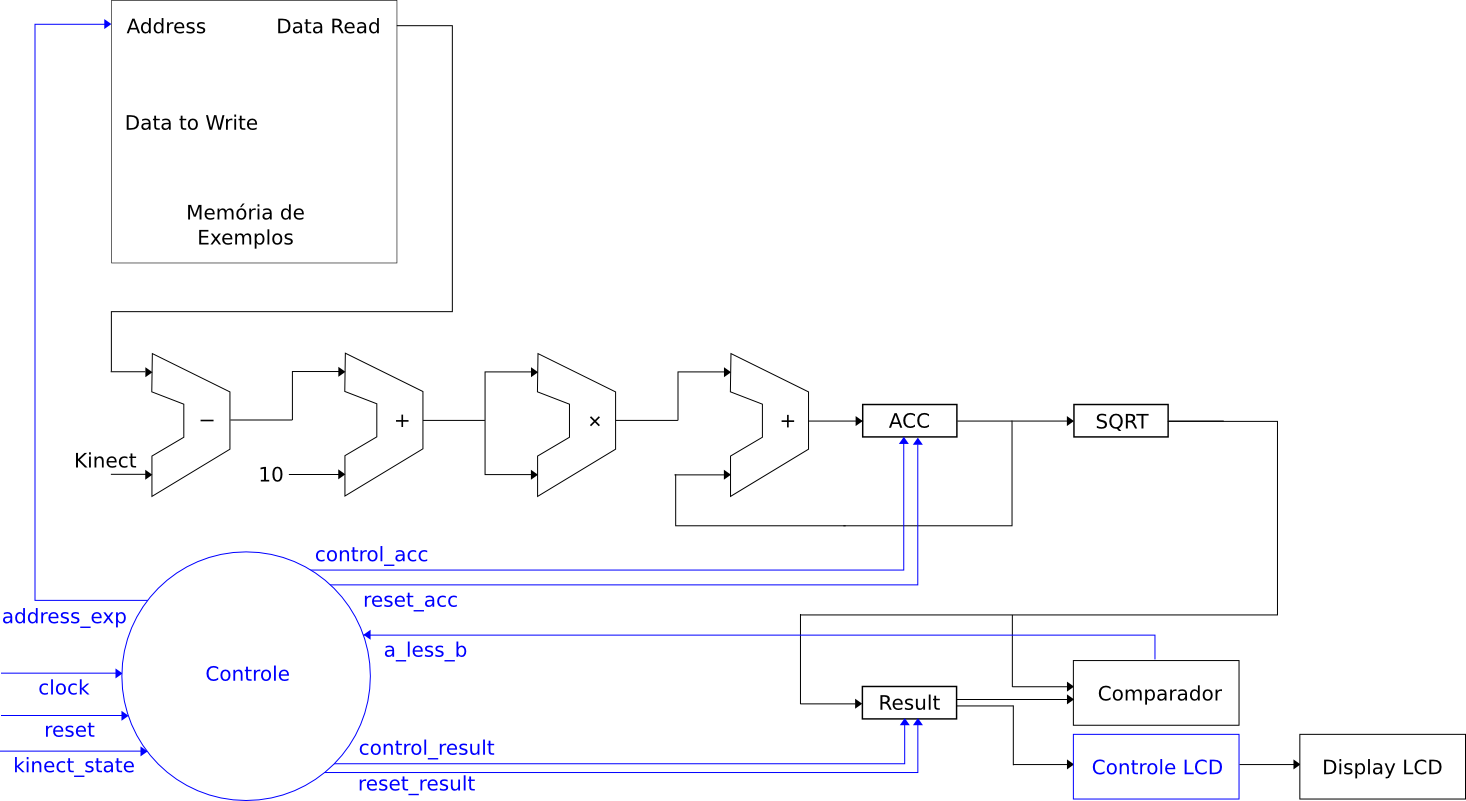
\includegraphics[scale=0.36]{img/circuito_knn.png}
\end{figure}

\begin{itemize}

\item \verb|adress_exp|:  Envia qual endereço da memória de exemplos deve ser acessado;
\item \verb|control_acc|: Ativa a carga no registrador acumulador no estado acc load;
\item \verb|reset_acc|: Reseta o acumulador;
\item \verb|control_result|: Ativa a carga no registrador que registra o resultado final;
\item \verb|reset_result|: Reseta o registrador;
\item \verb|kinect_state|: Sinaliza quando o exemplo vindo do kinect está pronto para ser processado;
\item \verb|a_less_b|: Resultado da comparação do valor vindo do cálculo da distância euclideana com o valor armezenado no registrador;
\end{itemize} 


\section{Conclus\~ao}\label{sec:figs}

Este trabalho desenvolveu um algoritmo em VHDL que...

%(Figure~\ref{fig:exampleFig1}), otherwise justified and indented by 0.8cm on
%both margins, as shown in Figure~\ref{fig:exampleFig2}. The caption font must

%\begin{figure}[ht]
%\centering
%\includegraphics[width=.5\textwidth]{fig1.jpg}
%\caption{A typical figure}
%\label{fig:exampleFig1}
%\end{figure}

%\begin{figure}[ht]
%\centering
%\includegraphics[width=.3\textwidth]{fig2.jpg}
%\caption{This figure is an example of a figure caption taking more than one
%  line and justified considering margins mentioned in Section~\ref{sec:figs}.}
%\label{fig:exampleFig2}
%\end{figure}

%\begin{table}[ht]
%\centering
%\caption{Variables to be considered on the evaluation of interaction
%  techniques}
%\label{tab:exTable1}
%\includegraphics[width=.7\textwidth]{table.jpg}
%\end{table}

%Bibliographic references must be unambiguous and uniform.  We recommend giving
%the author names references in brackets, e.g. \cite{knuth:84},
%\cite{boulic:91}, and \cite{smith:99}.

%The references must be listed using 12 point font size, with 6 points of space
%before each reference. The first line of each reference should not be
%indented, while the subsequent should be indented by 0.5 cm.

\bibliographystyle{sbc}
\bibliography{knn}

\end{document}
